% Chapter Template

\chapter{Long Range Communication Architecture} % Main chapter title

\label{Chapter3} % Change X to a consecutive number; for referencing this chapter elsewhere, use \ref{ChapterX}

\lhead{Chapter 3. \emph{Long Range Communication}} % Change X to a consecutive number; this is for the header on each page - perhaps a shortened title

In this chapter, we shall look at the long range communication architecture, menat for communication between ground station and the UAVs, and how it is integrated with the mesh network and ROS.

\section{Hardware}
Among the existing solutions for long range communication, radios based on 900Mhz spectrum seem popular. Compared to 2.4Ghz radios, there are a few reasons for this. First, the path loss for 2.4Ghz radios is higher than that of 900Mhz radios, reducing the received signal strength significantly over long distances. With the use of high gain directional antennas, the gap in the received signal strength between the radios of two spectra, can be eliminated, or even reversed. While this makes the 2.4Ghz radios favorable than 900Mhz radios in static point-to-point links, 900Mhz radios still have a much longer range than 2.4Ghz radios. Second, the 2.4Ghz spectrum is more vulnerable to the issues of penetration and blockages in the face of obstacles, while 900Mhz is more robust to them.

Note that much of 2.4Ghz hardware consists of wifi based solutions, based on the 802.11 hardware, and 802.11 was designed to be indoor, with short range, but high bandwidth. Consequently, hardware based on 802.11 is inefficient for use over long distances. While there are implementations of custom protocol stacks, instead of 802.11, on 2.4Ghz spectrum, these are almost always propietary and consequently, the modules are quite expensive. Considering all things, 900Mhz radios are still offer quite a promising solution for communication over long distances. One downside is that the 900Mhz radios typically offer lower bandwidth on the order of a few 100 Kbps, compared to 2.4Ghz solutions. Nonetheless, this should not be a problem as long as not too much data is demanded at the ground station, which is true in most applications.

\subsection{RFD900X}
RFD900X is third in line of popular 900Mhz radios by the company, RFDesign, the first two being RFD900 and RFD900+. The radio operates on frequency range 902-928 Mhz. It allows selectable transmit power upto 30dBm, in steps of 1dBm. It supports multiple air data rates from 4Kbps to 500Kbps. It has a UART interface supporting multiple baud rates from 9600 to 1000000. It has an advertised range of more than 50Kms in line of sight conditions, depending on antennas. The radios support a set of AT commands for configuring different parameters. There is decent documentation regarding the radios that can be found at \url{http://files.rfdesign.com.au/docs/}.

\begin{figure}[h]
	\centering
	\begin{subfigure}{0.5\textwidth}
		\centering
		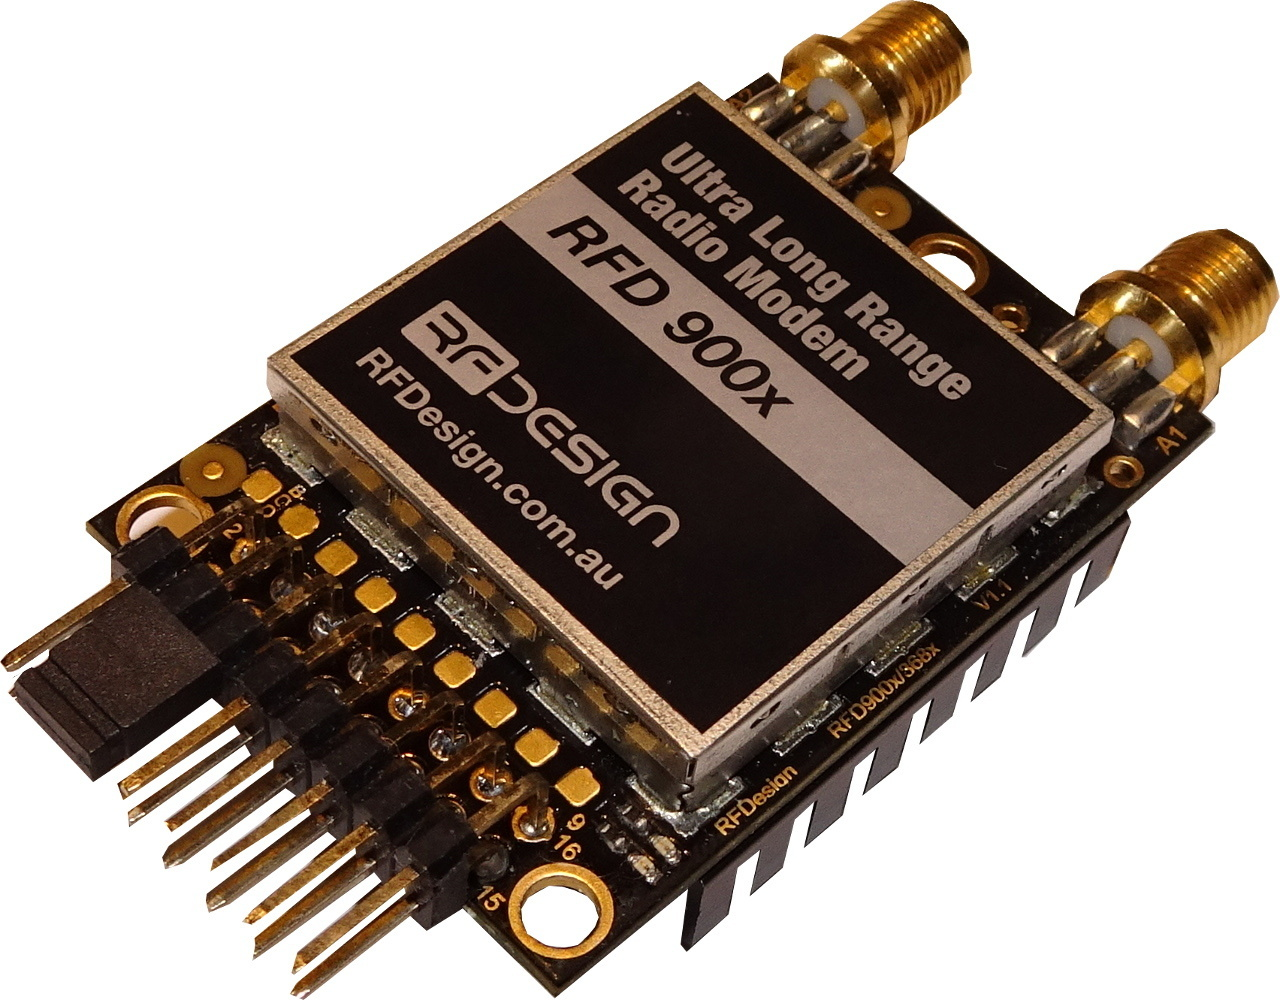
\includegraphics[scale=0.1]{Pictures/rfd1.jpg}
	\end{subfigure}%
	\begin{subfigure}{0.5\textwidth}
		\centering
		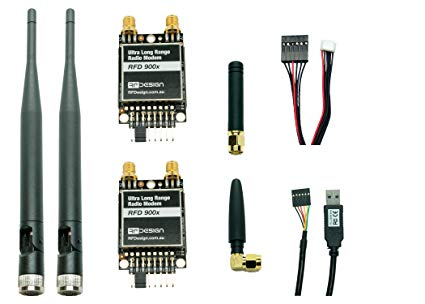
\includegraphics[scale=0.5]{Pictures/rfd2.jpg}
	\end{subfigure}
	\caption{RFD900x along with antennas and FTDI cables}
	\label{fig: rfd900x}
\end{figure}

The radios come with a default peer to peer firmware, which means that the radios can only be used in pairs. There are two other firmwares that can be flashed on radios, synchronous mesh and asynchronous mesh, which are point to multipoint firmwares. These firmwares can be flashed by a gui program called 'Modem Tools' that can downloaded from \url{http://files.rfdesign.com.au/}.

\subsubsection{Peer to Peer Firmware}
As mentioned, the radios come flashed with the peer to peer firmware by default. We may need to configure the radios with some parameters via the AT commands. For instance, the parameters NETID, SERIAL\_SPEED, AIR\_SPEED should be same on both the modems, among other things. Radios with same NETID can talk to each other. Essentially, any raw bytes input to the serial UART interface at one radio can be received at the serial interface of the other radio. Different pairs of radios with different NETIDs can only send and receive data to and from the radio with the same NETID. Even though you can have multiple pairs of radios wiht different NETIDs, as the total number of radios increase, interference also increases, increasing the errors in transmitted bytes.

\begin{figure}[h]
	\centering
	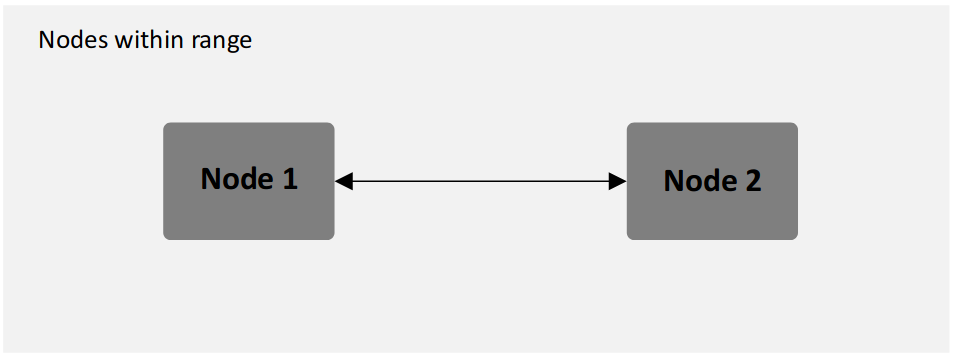
\includegraphics[scale=0.4]{Pictures/peer.png}
	\caption{modems in peer to peer configuration}
	\label{fig: rfdpeer}
	\captionsetup{font={footnotesize,bf,it}}
	\caption*{source: http://files.rfdesign.com.au/Files/documents/RFD900x\%20DataSheet\%20V1.1.pdf}
\end{figure}

\subsubsection{Synchronous Mesh Firmware}
While the peer to peer firmware allows communication only between a pair of radios, the asynchronous firmware is a point to multipoint firmware. Apart from the NETID parameter, there is a NODEID parameter, NODEDESTINATION parameter, NETCOUNT parameter among others, that can be set by the AT commands. Unlike the peer to peer firmware, more than two radios can have the same NETID. While using the synchronous firmware, one of the radios needs to be as a base node. This can be done by setting the NETID parameter to 0 and NODEID parameter to 1 on the base radio. We should also specify the number of radios with the parameter NETCOUNT.

In this configuration, the base radio assigns time slots to each of the other radios to communicate. Essentially, each radio transmits data only during its assigned time slot. So, even if other radios are not transmitting data, a radio waits for its time slot to transmit its data. This is inefficient when either not many radios are transmitting or they are not transmitting too often.

\begin{figure}[h]
	\centering
	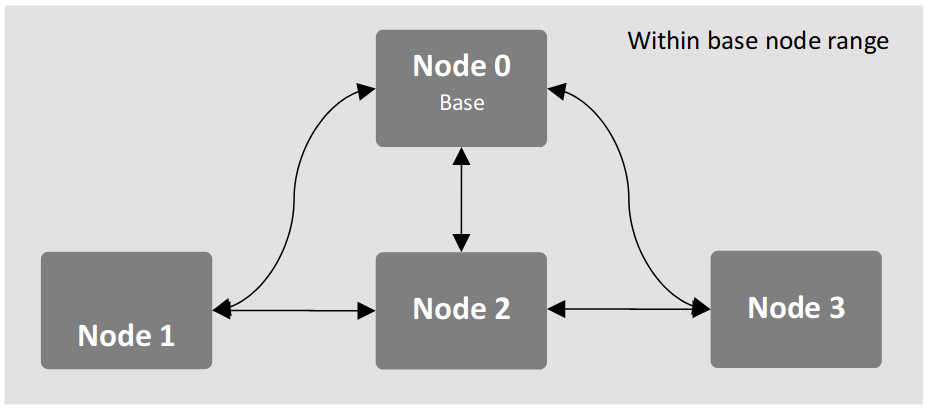
\includegraphics[scale=0.4]{Pictures/sync.png}
	\caption{modems in synchronous mesh configuration}
	\label{fig: rfdsync}
	\captionsetup{font={footnotesize,bf,it}}
	\caption*{source: http://files.rfdesign.com.au/Files/documents/RFD900x\%20DataSheet\%20V1.1.pdf}
\end{figure}




